\documentclass{article}

\usepackage[portuguese]{babel}
\usepackage[utf8]{inputenc}
\usepackage[letterpaper,top=2cm,bottom=2cm,left=3cm,right=3cm,marginparwidth=1.75cm]{geometry}
\usepackage{amsmath}
\usepackage{graphicx}
\usepackage[colorlinks=true, allcolors=blue]{hyperref}
\usepackage{listings}
\usepackage{xcolor}
\usepackage{cite}
\usepackage{float}
\usepackage{lipsum}
\usepackage{tabularx}
\usepackage{pdflscape}
\usepackage{setspace}
\setstretch{1.5}
\lstset{
  language=Python,
  basicstyle=\ttfamily\small,
  numbers=left,
  numberstyle=\tiny\color{gray},
  keywordstyle=\color{blue},
  commentstyle=\color{gray},
  stringstyle=\color{orange},
  breaklines=true,
  frame=single,
  columns=flexible
}

\title{Avaliação 2 de Introdução a Computação}
\author{Nathan Loose Kuipper \\ Rafael Gontijo Ferreira}

\begin{document}
\maketitle

\begin{abstract}

\lipsum[1-2]  % Substituir
\end{abstract}
\pagebreak
\section{Introdução}
Este trabalho tem como objetivo analisar os dados contidos no arquivo \texttt{bilheteria.db}, referentes a sessões de cinema realizadas em diversos complexos no país. A partir dessas informações, foram respondidas as questões propostas, com a realização de agrupamentos e a geração de visualizações que fornecem \textit{insights} sobre a exibição e o consumo de filmes no Brasil. Utilizando a linguagem \texttt{Python} e bibliotecas como \texttt{pandas}, \texttt{matplotlib} e \texttt{seaborn}, foi feita a limpeza e análise dos dados, além da construção de tabelas e gráficos que facilitam a compreensão do cenário cinematográfico nacional.

\section{Análise do Código}
Nesta seção, cada aspecto que compõe a Parte Um do trabalho será analisado de forma minuciosa, ou seja, as cinco questões propostas e os módulos de apoio apresentados.
\subsection*{Módulo Auxiliar A2}
Além das funções apresentadas no caderno Jupyter, \texttt{carrega\_tabela} e \texttt{lista\_tabelas}, foi também implementada a função \texttt{queryconn}, que recebe como parâmetros a base de dados e a consulta SQL. Essa função permite a execução de \textit{queries} de forma mais flexível, facilitando alterações e prototipagens durante o desenvolvimento.
\linespread{1}
\begin{lstlisting}
AUTORES = ['Nathan Loose Kuipper', 'Rafael Gontijo Ferreira']

import pandas as pd 
import sqlite3
from pathlib import Path

PATH =  Path(__file__).parent # bilheteria.db na mesma pasta que esse arquivo

def queryconn(database, query):
    with sqlite3.connect(database) as conn:
        cursor = conn.cursor()
        cursor.execute("SELECT name FROM sqlite_master WHERE type='table';")
        tables = cursor.fetchall()

        df = pd.read_sql_query(query, conn)
        
        return df
    
def carrega_tabela(database, tabela):

    ...

def lista_tabelas(db_filename):

   ...
    
if __name__ == '__main__':
    print("Importe esse modulo para auxilar com o manejo da base de dados!")
\end{lstlisting}
\linespread{1.5}
\subsection*{Questão 1}
Na \textbf{Questão 1}, foi utilizado o método \texttt{groupby()} para agrupar os dados por \texttt{filme\_id} e calcular a soma do público com \texttt{sum()}. O método \texttt{reset\_index()} foi aplicado para transformar o índice em coluna. A função \texttt{map()} foi usada para substituir os IDs dos filmes pelos respectivos títulos, com apoio do método \texttt{loc[]}.
\linespread{1}
\begin{lstlisting}
def questao1():
    
    dsessao = a2.carrega_tabela(PATH / 'bilheteria.db', 'sessao')
    dfsessao = dsessao.groupby(by=['filme_id'])['publico'].sum().reset_index()

    dfilme = a2.carrega_tabela(PATH / 'bilheteria.db', 'filme')
    
    map_titulo = lambda x: dfilme.loc[dfilme['id'] == x, 'titulo_original'].item()
    dfsessao['filme_id'] =  dfsessao['filme_id'].map(map_titulo).astype(str)
    
    return dfsessao
\end{lstlisting}
\linespread{1.5}
\subsection*{Questão 2}
Na \textbf{Questão 2}, novamente foi usado \texttt{groupby()} com \texttt{sum()} para calcular o público total por filme. O método \texttt{merge()}\footnote{No método \texttt{merge()}, o parâmetro \texttt{left\_on} especifica a coluna da tabela esquerda usada para junção, enquanto \texttt{right\_on} indica a coluna correspondente da tabela direita. O parâmetro \texttt{how} determina o tipo de junção: \texttt{'left'} mantém todas as linhas da tabela esquerda, incorporando as correspondências da direita; \texttt{'right'} faz o oposto; \texttt{'inner'} retorna apenas as linhas correspondentes em ambas; e \texttt{'outer'} retorna todas as linhas de ambas as tabelas, preenchendo com \texttt{NaN} onde não há correspondência.} integrou os dados das sessões com a tabela de filmes. O \texttt{fillna(0)} garantiu que filmes sem sessões tivessem público zero. A ordenação foi feita com \texttt{sort\_values()} e a seleção do maior foi realizada com \texttt{iloc[0]}.
\linespread{1}
\begin{lstlisting}
  def questao2():
    dfilme = a2.carrega_tabela(PATH / 'bilheteria.db', 'filme')
    dsessao = a2.carrega_tabela(PATH / 'bilheteria.db', 'sessao')
    dfsessao = dsessao.groupby(by=['filme_id'])['publico'].sum().reset_index()
    merged_df = dfilme.merge(dfsessao, left_on='id', right_on='filme_id', how='left')
    merged_df['publico'] = merged_df['publico'].fillna(0)
    
    paises = merged_df['pais_origem'].unique()
    dic = {}
    
    for pais in paises:
        most_viewed_film = merged_df[merged_df['pais_origem'] == pais].sort_values(by='publico', ascending=False).iloc[0]
        dic[pais] = {
            'nome': dfilme.loc[dfilme['id'] == most_viewed_film['filme_id'], 'titulo_original'].item(),
            'publico': int(most_viewed_film['publico'])
        }
    
    return dic
\end{lstlisting}

\linespread{1.5}
\pagebreak
\subsection*{Questão 3}
Na \textbf{Questão 3}, o método \texttt{merge()} foi usado para unir as tabelas \texttt{sessao}, \texttt{sala} e \texttt{complexo}. O agrupamento por cidade foi feito com \texttt{groupby()} seguido de \texttt{sum()}. O resultado foi ordenado de forma decrescente com \texttt{sort\_values()} e limitado às 100 primeiras linhas com \texttt{head(100)}.
\linespread{1}
\begin{lstlisting}
    def questao3():
    
    dsessao = a2.carrega_tabela(PATH / 'bilheteria.db', 'sessao')
    dsala = a2.carrega_tabela(PATH / 'bilheteria.db', 'sala')[['id', 'from_complexo']]
    dcomplexo = a2.carrega_tabela(PATH / 'bilheteria.db', 'complexo')[['id', 'municipio']]

    df = dsessao.merge(dsala, left_on='sala_id', right_on='id', how='left')

    # junta o dataframe anterior com o dcomplexo para obter as cidades
    df = df.merge(dcomplexo, left_on='from_complexo', right_on='id', how='left')

    cidades = df.groupby('municipio', as_index=False)['publico'].sum()

    cidades = cidades.rename(columns={'publico': 'BILHETERIA'})

    top100 = cidades.sort_values('BILHETERIA', ascending=False).head(100)

    return top100
\end{lstlisting}
\linespread{1.5}
\subsection*{Questão 4}
Na \textbf{Questão 4}, as tabelas foram integradas usando \texttt{merge()}. O método \texttt{rename()} foi aplicado para ajustar os nomes das colunas. O agrupamento por cidade e filme usou \texttt{groupby()} com \texttt{sum()}, seguido de uma ordenação com \texttt{sort\_values()} e seleção do filme de maior bilheteria em cada cidade usando \texttt{groupby().head(1)}.
\linespread{1}
\begin{lstlisting}
    def questao4():
    
    dsessao = a2.carrega_tabela(PATH / 'bilheteria.db', 'sessao')
    dsala = a2.carrega_tabela(PATH / 'bilheteria.db', 'sala')[['id', 'from_complexo']]
    dcomplexo = a2.carrega_tabela(PATH / 'bilheteria.db', 'complexo')[['id', 'municipio']]
    dfilme = a2.carrega_tabela(PATH / 'bilheteria.db', 'filme')[['id', 'titulo_original']]

    df = dsessao.merge(dsala, left_on='sala_id', right_on='id', how='left')
    df = df.rename(columns={'id_x': 'sessao_id', 'id_y': 'sala_id'})  

    df = df.merge(dcomplexo, left_on='from_complexo', right_on='id', how='left')
    df = df.rename(columns={'municipio': 'CIDADE'})
    
    df = df.merge(dfilme, left_on='filme_id', right_on='id', how='left')
    df = df.rename(columns={'titulo_original': 'FILME'})

    bilheteria = df.groupby(['CIDADE', 'FILME'], as_index=False)['publico'].sum()
    bilheteria = bilheteria.rename(columns={'publico': 'BILHETERIA'})

    resultado = bilheteria.sort_values('BILHETERIA', ascending=False).groupby('CIDADE').head(1)

    return resultado[['CIDADE', 'FILME', 'BILHETERIA']]

\end{lstlisting}

\subsection*{Questão 5}
\linespread{1.5}
Na \textbf{Questão 5}, além de \texttt{merge()} e \texttt{rename()}, foi criada uma nova coluna \texttt{tipo} com o método \texttt{apply()} e uma função \texttt{lambda} para classificar os filmes como \texttt{BR} ou \texttt{ESTRANGEIRO}. Após o \texttt{groupby()} por cidade e tipo de filme, os dados foram reorganizados com \texttt{pivot()} e os valores nulos tratados com \texttt{fillna(0)}.
\linespread{1}
\begin{lstlisting}
    def questao5():
    
    dsessao = a2.carrega_tabela(PATH / 'bilheteria.db', 'sessao')
    dsala = a2.carrega_tabela(PATH / 'bilheteria.db', 'sala')[['id', 'from_complexo']]
    dcomplexo = a2.carrega_tabela(PATH / 'bilheteria.db', 'complexo')[['id', 'municipio']]
    dfilme = a2.carrega_tabela(PATH / 'bilheteria.db', 'filme')[['id', 'pais_origem']]

    df = dsessao.merge(dsala, left_on='sala_id', right_on='id', how='left')
    df = df.rename(columns={'id_x': 'sessao_id', 'id_y': 'sala_id'})

    df = df.merge(dcomplexo, left_on='from_complexo', right_on='id', how='left')
    df = df.rename(columns={'municipio': 'CIDADE'})

    df = df.merge(dfilme, left_on='filme_id', right_on='id', how='left')

    df['tipo'] = df['pais_origem'].apply(lambda x: 'BR' if isinstance(x, str) and 'BRASIL' in x else 'ESTRANGEIRO')

    bilheteria = df.groupby(['CIDADE', 'tipo'], as_index=False)['publico'].sum()

    tabela_final = bilheteria.pivot(index='CIDADE', columns='tipo', values='publico').fillna(0)

    tabela_final = tabela_final.rename(columns={'BR': 'BILHETERIA_BR', 'ESTRANGEIRO': 'BILHETERIA_ESTRANGEIRA'}).reset_index()
    

    return tabela_final

\end{lstlisting}
\pagebreak
\section*{Visualizações}
\subsection*{Visualização 1:}
\begin{figure}[H]
    \centerline{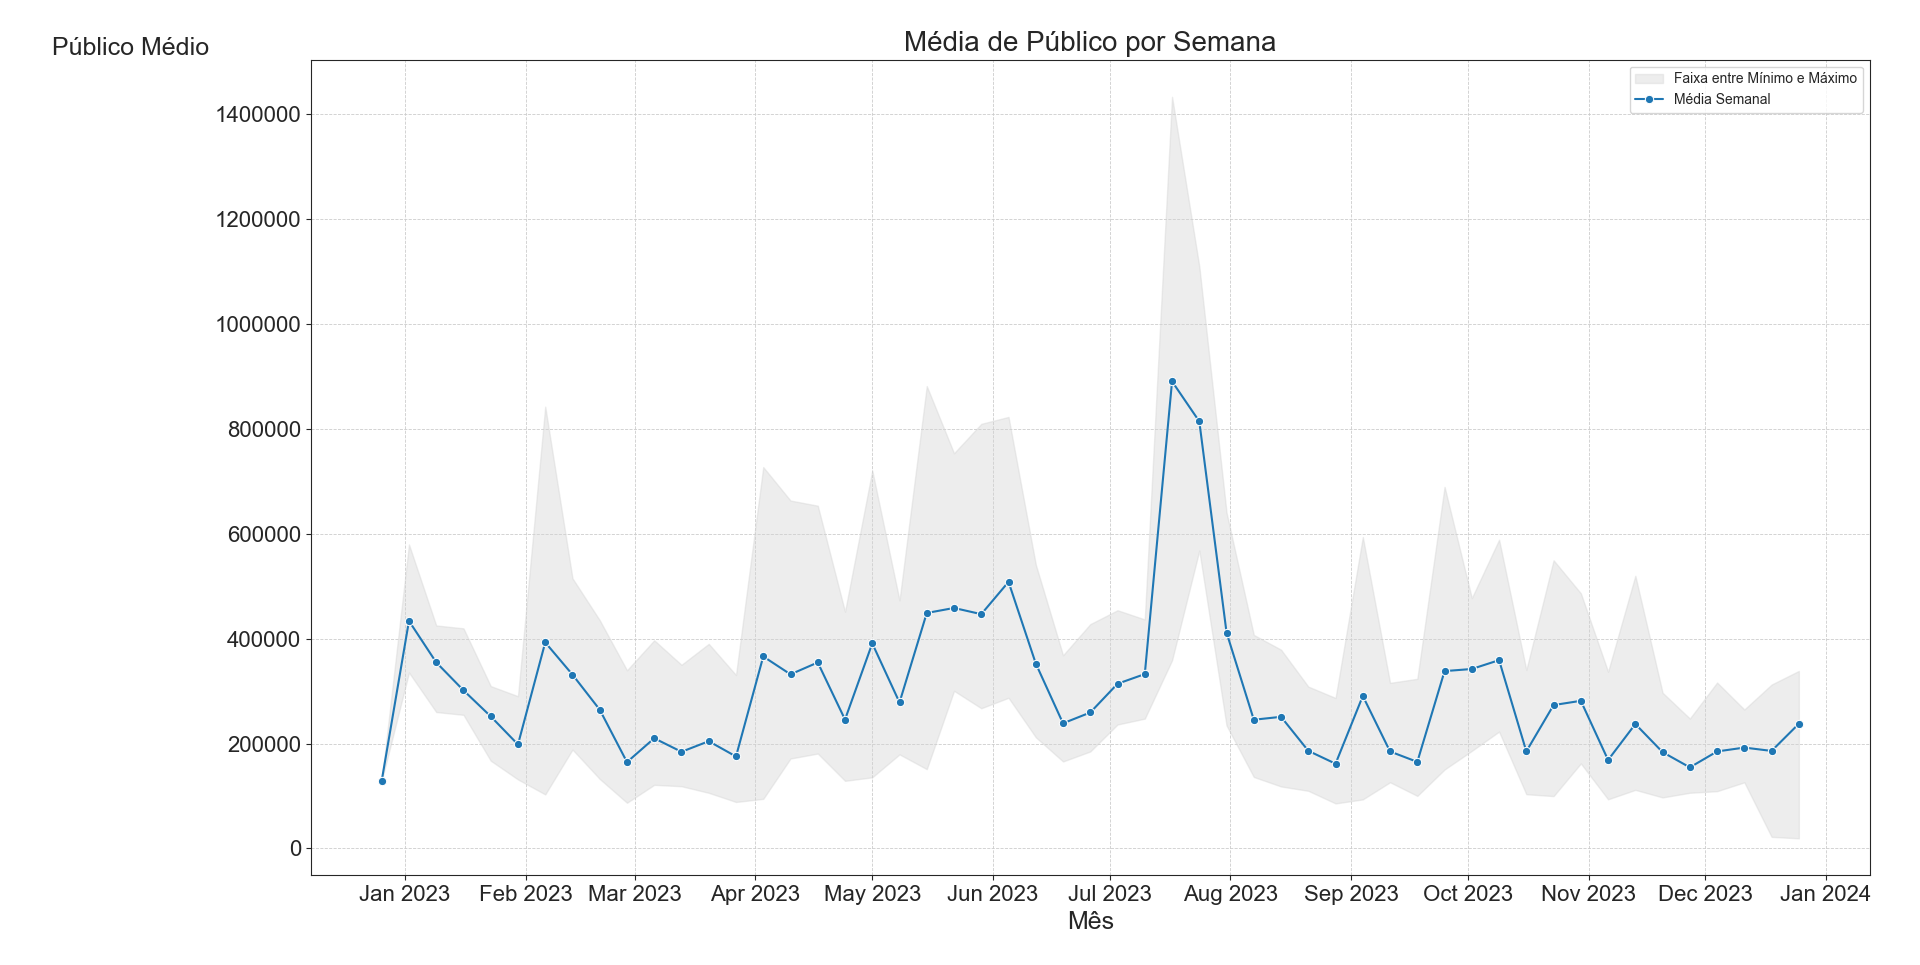
\includegraphics[width =\linewidth]{img/Figure_1.png}}
\end{figure}

A Visualização acima apresenta a variação da média semanal de público ao longo do ano de 2023. O gráfico de linha exibe o valor médio de público registrado por semana, enquanto a faixa sombreada representa o intervalo entre os valores mínimo e máximo observados no período, oferecendo uma ideia da dispersão dos dados. É possível observar que o público apresenta grandes autos e baixos ao longo do ano, sugerindo que terá um grande público nas estreias de grandes filmes ou feriados prolongados Como observado em julho.
\subsection*{Visualização 2:}
\begin{figure}[H]
    \centerline{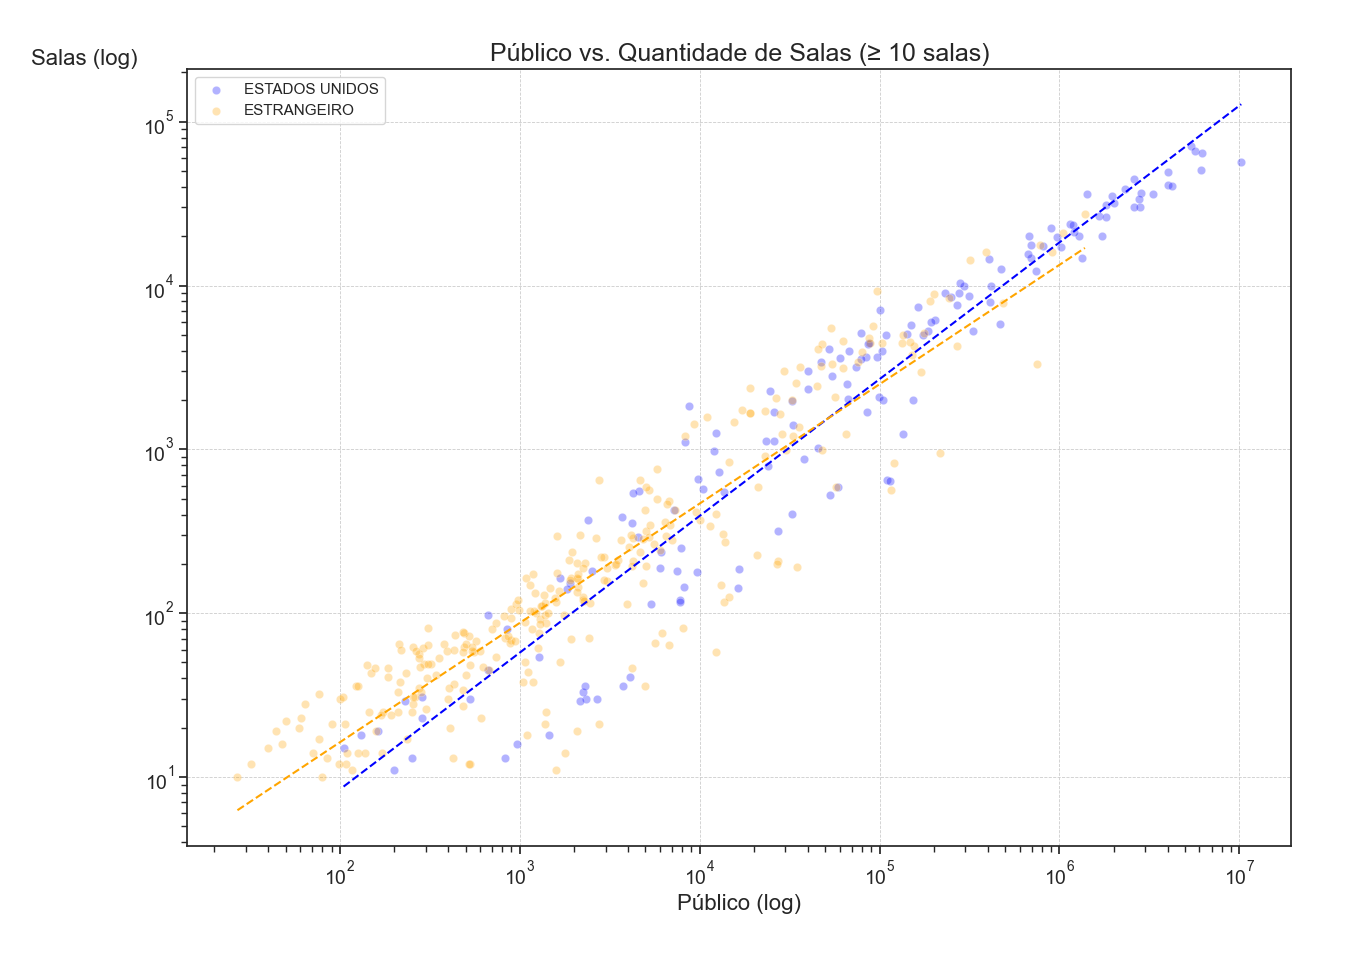
\includegraphics[width = \linewidth]{img/Figure_2.png}}
\end{figure}

A visualização acima relaciona o número de salas em que um filme foi exibido e o seu público total, considerando apenas filmes exibidos em 10 salas ou mais. Com ele, pode-se observar que quanto mais salas um filme ocupa, maior tende a ser o público.



O modelo de regressão linear no espaço logarítmico é dado por:

\[
\log_{10}(y) = a \cdot \log_{10}(x) + b
\]

onde:
\begin{itemize}
    \item \(y\) representa a quantidade de salas,
    \item \(x\) representa o público,
    \item \(a\) é o coeficiente angular (inclinação) da reta,
    \item \(b\) é o intercepto da reta.
\end{itemize}

\bigskip

A transformação para o espaço original é dada por:

\[
y = 10^{b} \cdot x^{a}
\]
\[
\min_{a,b} \sum_{i} \left( \log_{10}(y_i) - \left(a \cdot \log_{10}(x_i) + b \right) \right)^2
\]

onde \(\{(x_i, y_i)\}\) são os dados observados com \(x_i, y_i > 0\).

\subsection*{Visualização 3:}
\begin{figure}[H]
    \centerline{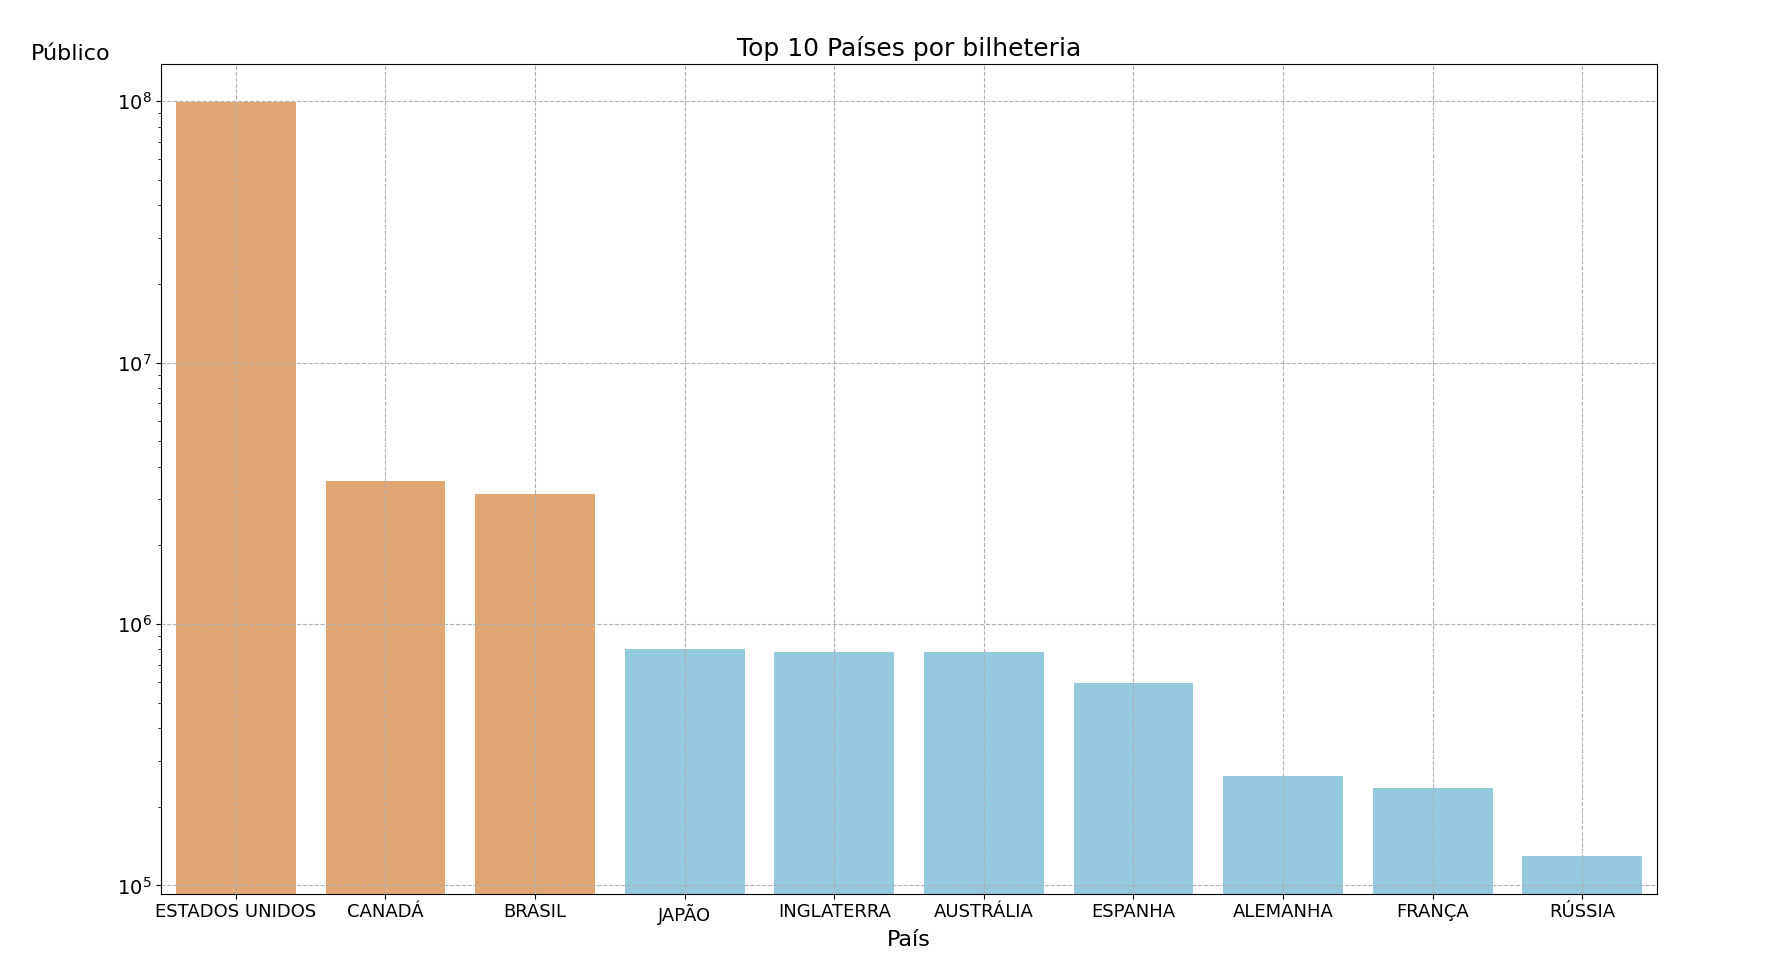
\includegraphics[width = \linewidth]{img/Figure_3.png}}
\end{figure}

A visualização apresentada foi dividida em dois gráficos de barras horizontais, à esquerda, podemos comparar a bilheteria do cinema brasileiro no cenário global\\
enquanto no da direita podemos comparar no cenário nacional.


Vale ressaltar que foi destacado com uma cor diferente o Brasil no primeiro gráfico e no segundo destacamos os três primeiros. Para que assim, possamos garantir uma\\
visualização mais clara e objetiva para quem irá vê-la.

\subsection*{Visualização 4:}
\begin{figure}[H]
    \centerline{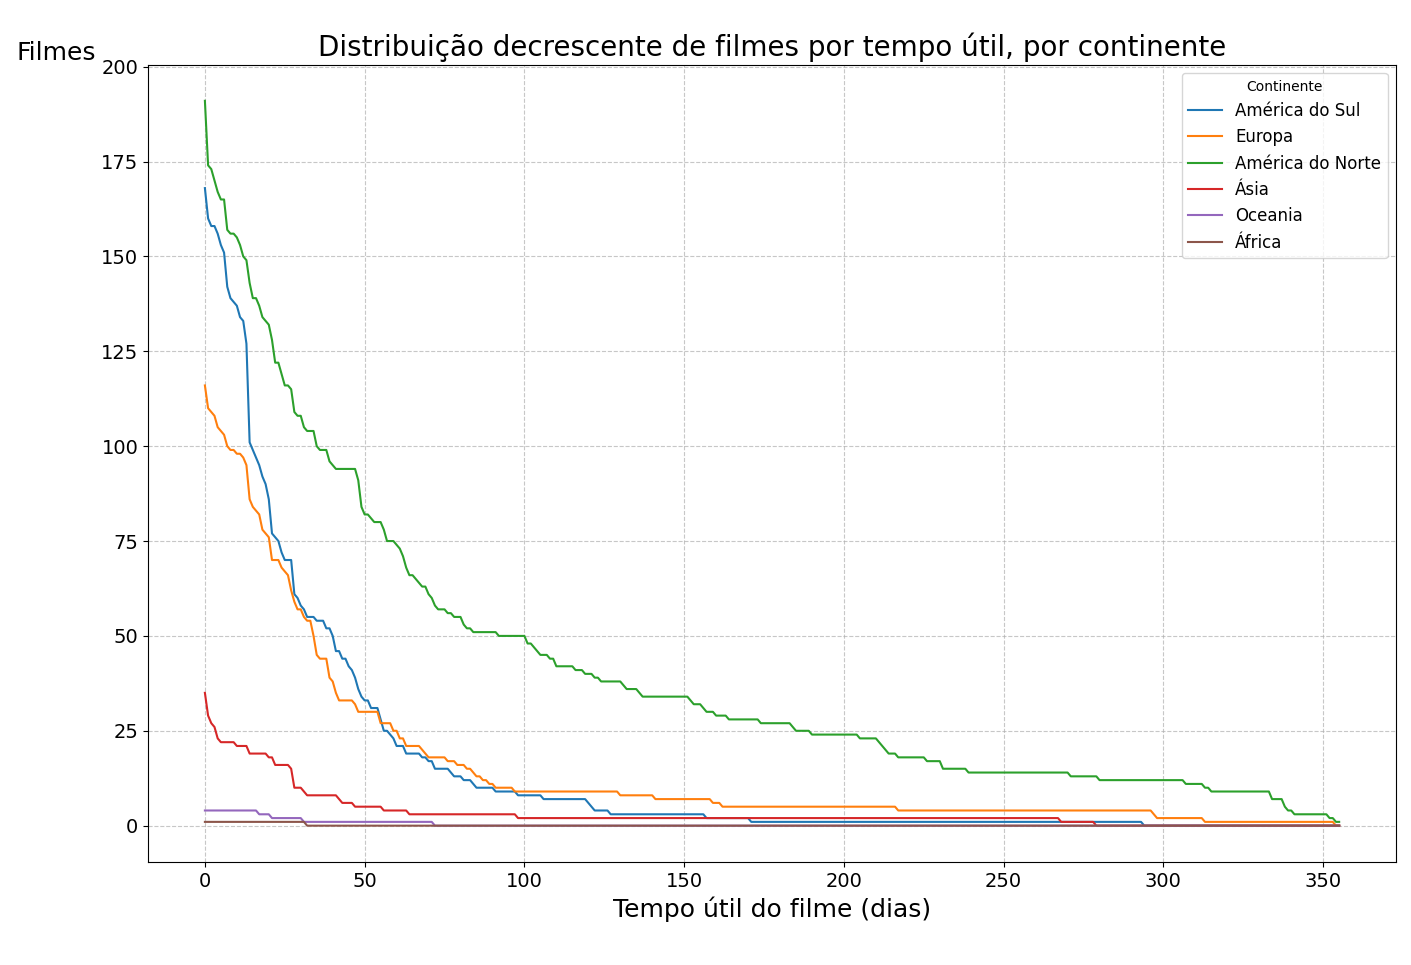
\includegraphics[width = \linewidth]{img/Figure_4.png}}
\end{figure}

Este gráfico de linha mostra a quantidade de filmes em função do tempo que permaneceram em cartaz, agrupados por continente. Com ele, é possível observar que a América do Norte possui uma indústria cinematográfica\\
com maior capacidade de sustentar filmes em exibição por longos períodos. Enquanto que em continentes como África e Oceania, os filmes tendem a ter ciclos de exibição mais curtos, refletindo limitações de mercado ou de distribuição.

\section*{Tabelas}

\subsection*{Tabela 1}

\begin{table}[H]
\centering
\caption{Tempo útil médio de exibição por país de origem}
\begin{small}
\begin{tabular}{l r}
\hline
\textbf{País de Origem} & \textbf{Tempo Útil Médio (dias)} \\
\hline
SUÉCIA & 161.00 \\
CHINA & 143.75 \\
BELARUS (BIELORUSSIA) & 129.00 \\
ESPANHA & 109.60 \\
IRÃ & 97.00 \\
ESTADOS UNIDOS & 75.43 \\
CANADÁ & 75.22 \\
POLÔNIA & 73.60 \\
ÁUSTRIA & 68.00 \\
BÉLGICA & 58.00 \\
COLÔMBIA & 58.00 \\
ALEMANHA & 55.44 \\
EMIRADOS ÁRABES UNIDOS & 55.00 \\
PANAMÁ & 54.00 \\
HOLANDA & 41.00 \\
\end{tabular}
\end{small}

\begin{center}
\small
\ldots
\end{center}

\end{table}
 
 Essa tabela apresenta o tempo útil médio (em dias) que os filmes permanecem em exibição nos cinemas,
agrupados por país de origem. Esse indicador permite avaliar a longevidade média das produções cinematográficas de cada país.

Com ela, pode-se notar que o tempo médio de exibição não segue estritamente o tamanho ou poder da indústria cinematográfica.
Isso porque, países menos centrais em termos de volume de produção podem ter filmes com maior longevidade. Enquanto grandes produtores,
como os EUA, mesmo com forte presença global, apresentam tempos mais moderados, possivelmente devido à maior rotatividade de lançamentos.

\pagebreak
\subsection*{Tabela 2}

\begin{table}[H]
\centering
\caption{Estatísticas de público por filme: média, desvio padrão, moda do dia da semana, semana do mês e mês de exibição}
\begin{small}
\begin{tabularx}{\textwidth}{X r r l c c}
\hline
\textbf{Título} & \textbf{Média Público} & \textbf{Desvio ($\sigma$)} & \textbf{Moda Dia} & \textbf{Moda Semana} & \textbf{Moda Mês} \\
\hline
FALE COMIGO & 227.83 & 299.91 & Quinta-feira & 3 & 8 \\
GODZILLA MINUS ONE & 227.07 & 216.66 & Quinta-feira & 2 & 12 \\
DECISÃO DE PARTIR & 211.83 & 231.45 & Quinta-feira & 2 & 1 \\
13 EXORCISMOS & 205.23 & 154.26 & Quinta-feira & 4 & 2 \\
BARBIE & 181.65 & 241.66 & Sábado & 4 & 8 \\
TRIÂNGULO DA TRISTEZA & 180.03 & 208.68 & Quinta-feira & 2 & 2 \\
THE CHOSEN... & 179.42 & 102.65 & Quinta-feira & 1 & 9 \\
TUDO EM TODO... & 169.97 & 197.06 & Quinta-feira & 3 & 3 \\
SAPATINHO VERMELHO... & 161.00 & --- & Quinta-feira & 3 & 4 \\
ENCANTO & 160.00 & --- & Quarta-feira & 2 & 12 \\

\end{tabularx}
\end{small}
\begin{center}
$\ldots$
\end{center}
\end{table}

Esta tabela apresenta um conjunto de estatísticas descritivas sobre o desempenho de diferentes 
filmes em termos de público. Os dados analisam a média de público, o desvio padrão, e a moda para três variáveis: dia, semana e mês do ano.

Nela, podemos observar que o filme "Fale comigo" apresenta a maior média de público (227,83), mas 
também o maior desvio padrão (299,91), indicando forte variação nas sessões.

\begin{landscape}
\subsection*{Tabela 3}
\begin{table}[H]
\centering
\small
\caption{Métricas de Exibição por Distribuidora}
\begin{tabular}{p{5cm}rrrrr}
\hline
\textbf{Distribuidora} & \textbf{Público} & \textbf{Total de Sessões} & \textbf{Média por Sessão} & \textbf{Desvio ($\sigma$)} & \textbf{Tempo Útil Médio (dias)} \\
\hline
WARNER BROS. (SOUTH) INC. & 52.935.246 & 688.130 & 76,93 & 116,40 & 96,24 \\
THE WALT DISNEY COMPANY (BRASIL) LTDA. & 24.273.591 & 341.583 & 71,06 & 89,57 & 83,76 \\
SM DISTRIBUIDORA DE FILMES LTDA & 9.547.406 & 195.485 & 48,84 & 70,37 & 30,52 \\
COLUMBIA TRISTAR FILMES DO BRASIL LTDA & 8.343.669 & 181.091 & 46,07 & 67,41 & 97,00 \\
PARAMOUNT PICTURES BRASIL DISTRIBUIDORA DE FILMES LTDA & 7.870.782 & 151.971 & 51,79 & 64,63 & 155,94 \\
DIAMOND FILMS DO BRASIL PRODUÇÃO E DISTRIBUIÇÃO DE FILMES LTDA & 1.993.412 & 22.267 & 89,52 & 161,46 & 36,24 \\
WMIX DISTRIBUIDORA LTDA. & 1.919.667 & 71.127 & 26,99 & 37,84 & 57,29 \\
VITRINE FILMES LTDA & 531.904 & 10.163 & 52,34 & 89,98 & 33,89 \\
ANTONIO FERNANDES FILMES LTDA & 444.162 & 9.968 & 44,56 & 56,83 & 46,80 \\
UNITED CINEMAS INTERNATIONAL BRASIL LTDA. & 357.937 & 8.165 & 43,84 & 60,57 & 9,80 \\
CINECOLOR DO BRASIL LTDA & 316.779 & 9.411 & 33,66 & 47,82 & 10,54 \\
FREESPIRIT DISTRIBUIDORA DE FILMES LTDA. & 225.561 & 11.002 & 20,50 & 27,08 & 40,25 \\
SA DISTRIBUIDORA DE CONTEÚDO AUDIOVISUAL LTDA & 216.849 & 955 & 227,07 & 216,66 & 27,00 \\
PLAYARTE PICTURES ENTRETENIMENTOS LTDA. & 191.989 & 10.282 & 18,67 & 23,70 & 25,40 \\
H2O DISTRIBUIDORA DE FILMES LTDA & 185.049 & 5.893 & 31,40 & 59,81 & 42,67 \\





\end{tabular}
\begin{center}
$\ldots$
\end{center}
\end{table}
\end{landscape}


Esta tabela fornece estatísticas que ajudam a entender o desempenho das principais distribuidoras 
de filmes no mercado, considerando tanto o volume de público quanto o padrão de exibição.Esses dados
são úteis para entender tanto o alcance quanto o comportamento de exibição dos filmes conforme a estratégia de distribuição adotada.

Nele podemos ver que quem lidera em todos os aspectos é a WARREN BROS. (SOUTH) INC, com ela
contendo o maior público, maior número de sessões, e o maior tempo útil médio.

\section*{Conclusão}

Através desse trabalho, podemos fazer uma análise abrangente sobre o desempenho da cinematografia ao redor do mundo,
com ênfase em métricas de bilheteria, tempo de exibição, distribuição geográfica e estratégias de distribuidoras.

Por meio das visualizações, podemos tirar conclusões muito interessantes, como a de que a quinta-feira aparece com 
destaque como o dia mais comum de estreia e exibição de pico, alinhando-se com as práticas tradicionais do setor cinematográfico. E que
filmes com maior média de público (como Fale Comigo e Godzilla Minus One) possuem também altos desvios, sugerindo sessões com grande variação de lotação.

Os dados também revelam que o mercado de cinema no Brasil possui forte concentração regional e disparidade na longevidade dos filmes,
especialmente quando comparado a outros países. Desse modo, a cinematografia brasileira mostra-se competitiva internacionalmente e com espaço para crescimento.

\begin{thebibliography}{99}

\bibitem{ref1}
Autor, A. (Ano). \textit{Título do Livro}. Editora.

\end{thebibliography}

\end{document}
